\documentclass[condensed]{union-cs-thesis}

\usepackage{graphicx}
\usepackage[hidelinks]{hyperref}
\usepackage{cite}
\usepackage{fancyref}
\usepackage{amsmath}
\usepackage{amsthm}
\usepackage{amssymb}


\graphicspath{ {./images/} }

%------------------------------------------------------------

\begin{document}

\title{Generative Models of Biological Ontogeny}
\author{Andrew Hilton}
\date{\today}
\maketitle

%------------------------------------------------------------

\begin{abstract}
  \makeabstract
  The idea that an organism's evolutionary history is reflected in its development from embryo to mature adult allows Biologists to gain insight into the phylogenetic development of a species by observing the morphological changes of an individual.  However this only allows for the observation of what changes occur, not the underlying cause for these changes.  Using Generative Encodings to model the development of morphologies, we hope to test the environmental and geometric constraints that led to the development of the unique morphology of Skate intestines.  This paper will discuss previous work done with generative encodings, as well as the work done in relation to this project specifically.
\end{abstract}

%------------------------------------------------------------

\section{Introduction}

\par
Within Biology Recapitulation Theory states ``Ontogeny recapitulates Phylogeny,'' meaning that the development of an individual within a species from its embryonic state to maturity (\emph{Ontogeny}) reflects the evolutionary development of the species as a whole (\emph{Phylogeny}).  The basis of this theory is derived from the observation that there is notable similarities between embryonic states of most complex organisms, but as they development, their morphologies begin to diverge.  The rate at which they differentiate themselves from each other is relative to our understanding of the evolutionary distance between species.
\footnote{Organisms that are phylogenetically similar will resemble each other further into their ontogeny than those which are relatively phylogenetically different}
\begin{figure}[h]
  \centering
  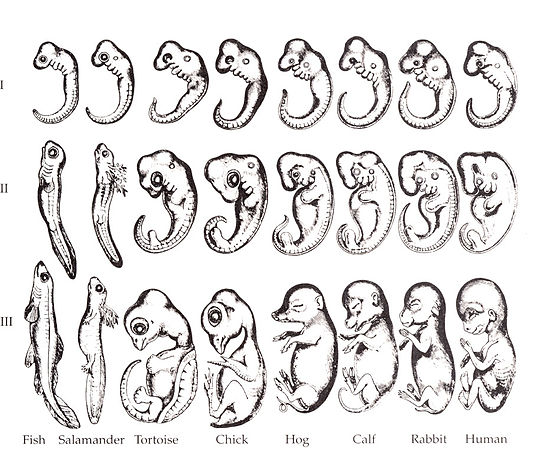
\includegraphics[width=.25\textwidth]{recapitulation}
  \caption{Ernest Haekel's diagram that initially inspired Recapitulation Theory}
  \label{fig:recapitulation_diagram}
\end{figure}
By using this principle, Biologists are able track the evolutionary history of a given species, by observing the morphological changes throughout its ontogeny, allowing for an approximation of the phylogeny of a group of organisms.

\par
One family of organimsms whose phylogeny is of some interest is the fmaily of fish \emph{Rajidae}, also known as skates (see figure~\ref{fig:skatepic}).
\begin{figure}[h]
  \centering
  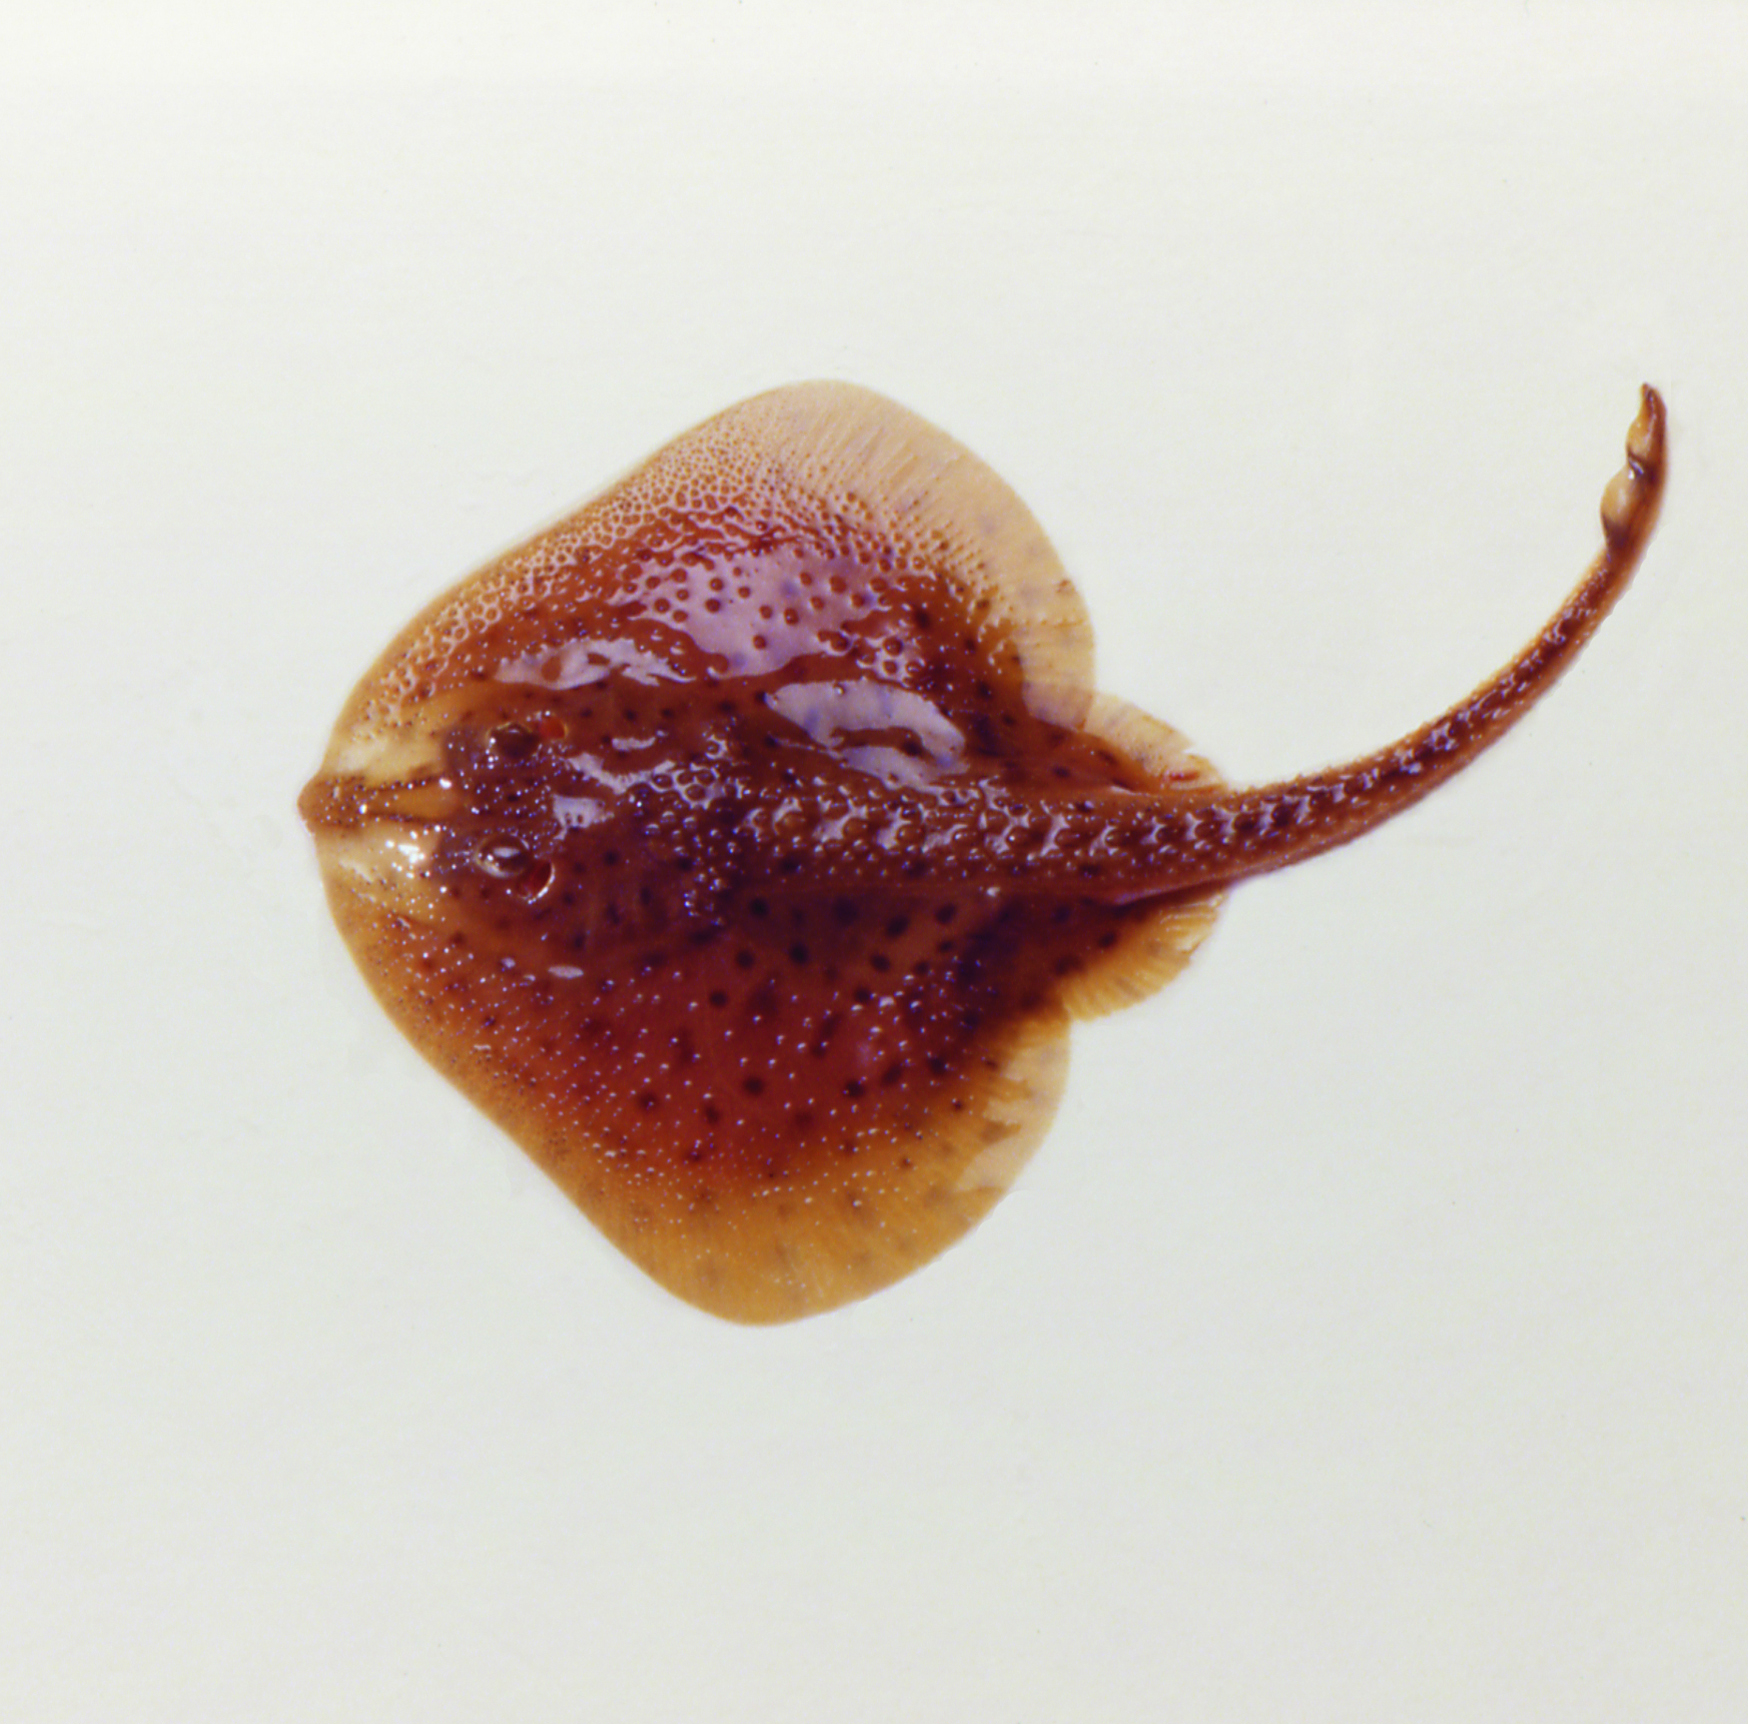
\includegraphics[width=.25\textwidth]{skate-pic}
  \caption{A mature skate specimen}
  \label{fig:skatepic}
\end{figure}
Skates are interesting from a biological and evolutionary standpoint largely due to their age (the predecessors to the modern Rajidae family are thought to have developed nearly 450 million years ago), meaning a lot of evolutionary history is encoded into their development, but also due to the fact that their intestinal tract has developed a unique morpholgy.  Like humans, skates' diets are protein rich.  Protein, by nature of its chemical structure, requires significant energy in order to break down into a usable form and digest.  One of the most successful strategies found in nature to solve this problem
\footnote{And the one used by Humans and our ancestors}
is the development of a long intestinal system, in order to increase the amount of surface area and therefore the rate of absorbtion within the gut.  The morphology of intestines in Humans and our predecessors is characterized by a long, thin tube more than twice our height, that coils around itself.  However the abdominal cavities of skates, which are cartilaginous fish, are not able to support this kind of structure.  As a result skate guts have developed into a contained volume with an internal spiral structure as opposed to a long tube coiled around itself (see figure~\ref{fig:gut_model}).
\begin{figure}[h]
  \centering
  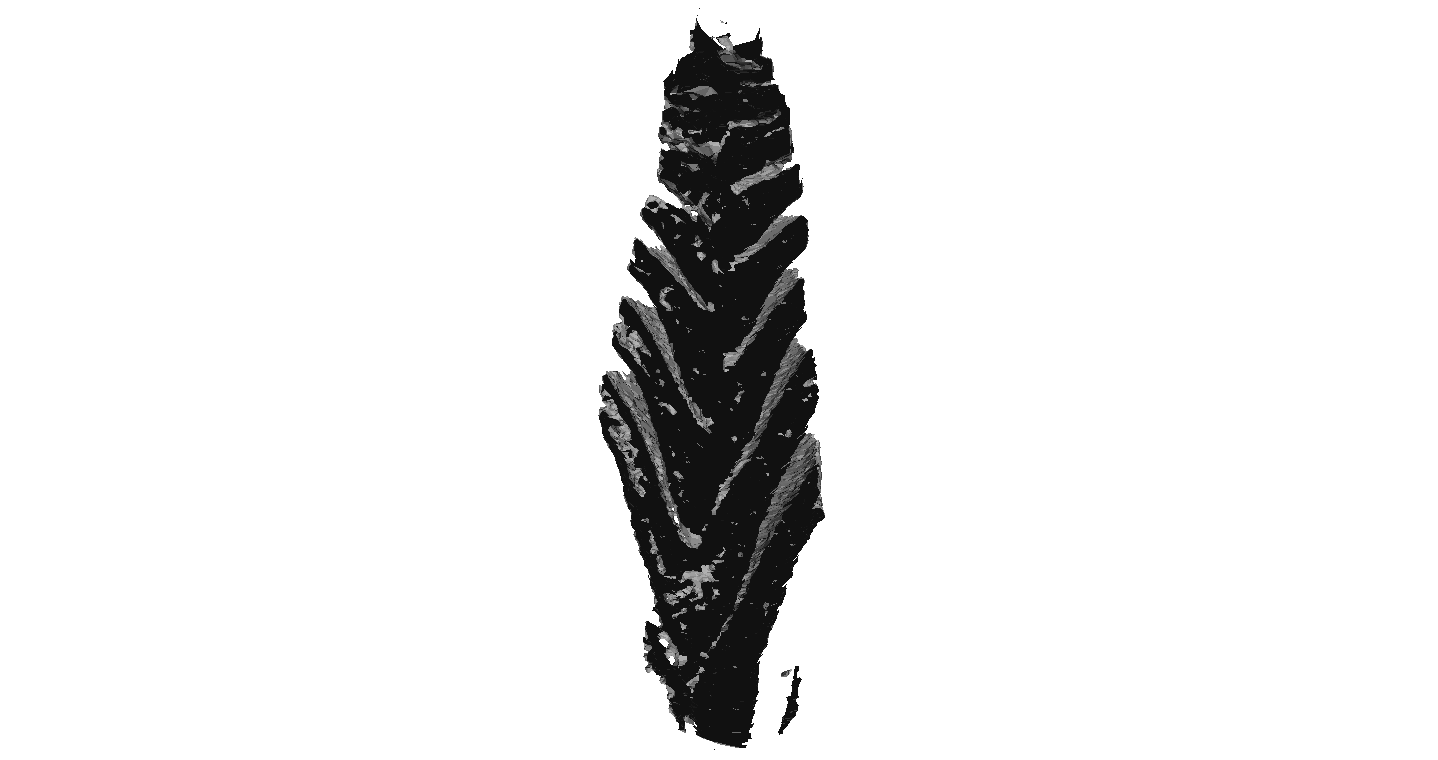
\includegraphics[width=.66\textwidth]{model_img}
  \caption{A 3D model of the internal membrane of a skate intestine, created trough CT-scans}
  \label{fig:gut_model}
\end{figure}

\par
The widely accepted explanations given for the development of this morphology are largely expressed in terms of geometric constraints and tied to this need for protein absorbtion.  While it is possible to infer these explanations given the biological needs of the skate, and the constraints imposed by the rest of its morphology, there is no way of directly testing these theories through traditional biological observations.  However using the principles of Recapitulation theory and Evolutionary Development, it may be possible to apply techniques of Evolutionary Computation in order to test the soundness and accuracy of these claims.  Using the parallels between Genetic Algorithms and Evolutionary Development as optimization searches for given measures of fitness as a basis, we will be applying Genetic Algorithms to the development of geometric models, and tailoring fitness functions in order to see if it is possible to produce morphologies similar to those seen in nature.

%------------------------------------------------------------

\section{Background \and Related Works}
\label{sec:background}

\par
While the use of Genetic Algorithms within the field of Computer Science is nothing new \cite{mitchell1998introduction}, and their applications are continually being tested and explored, their application to this particular problem space seems to be largely unexplored.  While GAs have been used in other areas of Biology, the application of GAs as a tool for investigating the physical constraints that lead to evolutionary development does not appear to have been extensively researched.  However a significant amount of research has gone into the potential of Generative Encodings.  Generative Encodings are a specific type of Genetic Algorithm, typically used in producing geometric models, that give the evolutionary system an understanding of specific strings within the genotype as ``genes'' and allow it to use encode the genetic instructions of solutions using these larger building blocks, and edit the makeup of genes globally\cite{toussaint2003demonstrating}.  Generative encodings have since been applied to area of soft-robotics in order to generate novel designs\cite{rieffel2009automated}, and have been used in order to optimize the design of antenae to be used on satellites\cite{lohn2005evolved}.  It has also been shown in the work done by Greg Hornby in evolving table designs, that the core concept behind Generative Encodings allows for the creation of novel designs of physical objects that are morphologically more interesting and generally more viable in terms of physical constraints than designs generated by naive sytems using direct encodings\cite{hornby2004functional,hornby2001advantages}.

\par
While the specific subproblem the work outlined in this paper is attempting to address, there has been work done within the field of Generative Encodings that bears some similarity to the type of problem space being investigated.  Marc Toussaint has done studies on the development of artificial plants, given biologically motivated measures of fitness\cite{toussaint2003demonstrating}.\footnote{In the case of Toussaint's work, investigating how exposure to the sun affects the resulting shape of a plant}  Toussaint's work has shown that using a Generative Encoding on an L-system grammar representation of artificial plants produces more effective solutions within fewer generations of a direct encoding.  The core of Toussaint's system was to allow for ``neutral mutations'' to occur, allowing different genotypes that express equivalent phenotypes to be substituted during the evolutionary process.  This resulted in multiple evolved shapes, of similar morphologies but distinct genetic representations to be produced, increasing the likelihood of evolving high-fitness solutions.

\par
The grammar based representation used in Toussaint's paper is of some interest to the work outlined here, as we wish to show the development of our shapes through time.  However the types of grammars used in Toussaint's lacks the geometric complexity\footnote{In terms of having 3D encapsulated volume, and surface area} to be fully useable for our work.  One type of grammar that fulfills many of the needs of this project is a tetrahedra-based face-encoding grammar, proposed by Rieffel et al. for use in the area of evolving biologically-inspired morphologies for soft-robotics \cite{Rieffel:face-grammar} (see figure~\ref{fig:tetra-blob}).
\begin{figure}[h]
  \centering
  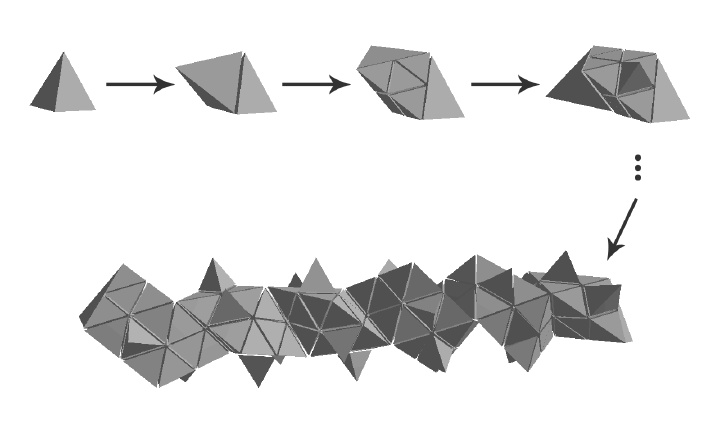
\includegraphics[width=.75\textwidth]{johngrammar}
  \caption{An example of the productions generated by this type of grammar}
  \label{fig:tetra-blob}
\end{figure}

%------------------------------------------------------------

\section{Methods and Design} \label{sec:work}


\subsection{Completed Work}

\emph{I think I could get a little bit more specific with some of my explanations, but I am right now most concerned with getting important information down}

\par
Much of the work done in the Fall term was towards implementing the grammar system, as well as being able to produce 3D models and renders of the shapes produced.  Admittedly too much time was spent trying to do the Math at the foundation of the system, when the solutions were finally discovered to be fairly simple, but heavily overlooked.  The system was implemented using Python 3, as this provides easy interfacing with Blender, which was the main software used to produce 3D models of the grammar productions.  Some modifications were made to the original grammar proposed by Rieffel et al., namely the removal of the Subdivide operation, as this results in an irregular polygon in the center of the tetrahedron that is not itself a tetrahedron.  The other major modification is the addition of the Rest operation, which itself just provides syntactic sugar for the operation.
\[A \to relabel(A)\]

\par
Following these modifications we have a grammar defined by the following operations
\begin{displaymath}
  \begin{matrix}
    rest()     \\
    relabel(A) \\
    grow(ABC)  \\
  \end{matrix}
\end{displaymath}
Where each $A,B,C$ are arbitrary labels within the grammar.

\emph{Around here is where I will put a diagram showing how the grow and relabel operations work}

\par
Following the implementation of the underlying grammar system, work was begun on generating 3D models of the grammar productions.  The primary tool used was Blender as it has an extensive Python API, but the system also has the ability to produce STL format files of the shapes for portability.

\subsubsection{Preliminary Results}
\par
By using the implemented systems, and writing a script that generated random grammar configurations, and produced 10 iterations of each grammar, we were able to produce some preliminary results showcasing the potential of the system.  While the initial pool of random grammars was quite small\footnote{Only including 15 different configurations} one of the configurations produced a geometrically interesting shape, known as Gram14 (see figure~\ref{fig:gram14}).\footnote{a 3D printed model of Gram14 was eventually produced}  Gram14 is produced after 10 iterations of the following grammar.
\begin{displaymath}
  \begin{matrix}
    A & \to & grow(CCA)  \\
    B & \to & rest()     \\
    C & \to & relabel(D) \\
    D & \to & grow(BBD)
  \end{matrix}
\end{displaymath}

\begin{figure}[h]
  \centering
  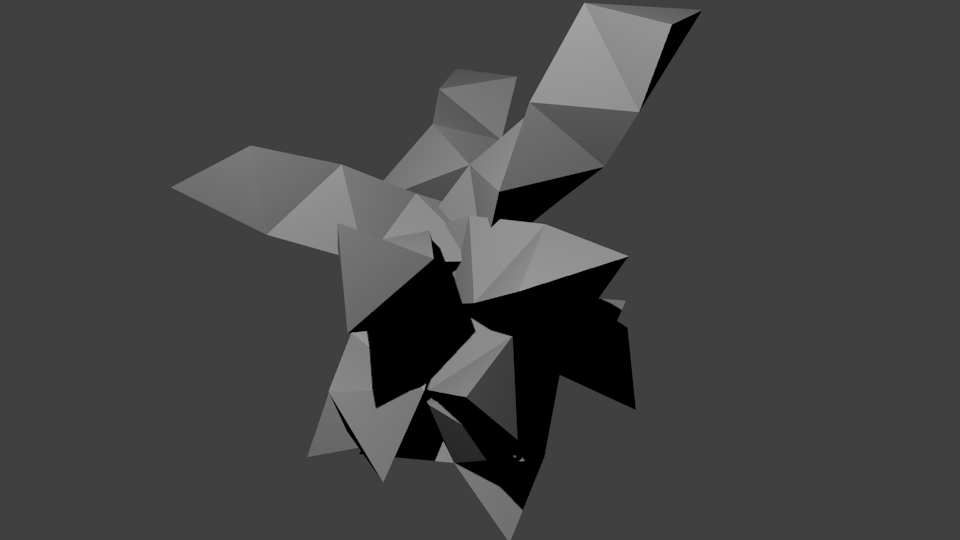
\includegraphics[width=.75\textwidth]{gram14}
  \caption{Gram14: The $i=10$ iteration of the 14th random grammar tested}
  \label{fig:gram14}
\end{figure}


\subsection{Outlining Procedure}

\par
Now that we have selected the system for generating the evolved shapes, and have substantial evidence that it is able to produce sufficiently ``interesting'' shapes, the overall design of our experiments is fairly trivial.\footnote{The specific implementation much less so}  The investigation will consist of
\begin{enumerate}
\item Creating a measure of fitness based on geometric constraints, motivated by Biological theories regarding the development of skate guts
\item Doing evolutionary runs of grammars using these fitness functions
\item Evaluating the shapes produced in order to see if any morphologies were generated that resemble shapes seen in nature
\end{enumerate}
The complexity of this procedure arises from the need to produce accurate fitness functions based on geometric constraints (and the method in which to collect this geometric data from our models), as well as the evaluation of our results.  While doing a qualitative evaulation is pretty trivial\footnote{``Does this shape \emph{look} like what is seen in nature}, creating a quantitative measure of the geometric similarity of models produced by our system and models generated from actual skate intestines requires a completely different and extensive approach (discussed in Section~\ref{sec:future}).

%------------------------------------------------------------

\section{Moving Forward} \label{sec:future}

\subsection{Fine-Tuning the Grammar}
While we were able to produce interesting shapes with the grammar there are some flaws and unwanted behavior that will have to be resolved before the system is fully ready to be used moving forward.  One of the main issues that will have to be addressed is the tendency for grammars with a lot of Grow operations to produce spherical formations, due to the lack of collision within the system itself.  As faces do not have an extensive understanding of other faces within the system, when many Grow operations are combined, faces begin to grow into each other producing shapes like those seen in Figure~\ref{fig:ball-gram}, which was produced by the grammar shown below.  Hopefully adding more robust collision detection to the system helps to reduce the occurences of these kinds of shapes.

\begin{displaymath}
  \begin{matrix}
    A & \to & grow(CBD)  \\
    B & \to & rest()     \\
    C & \to & grow(BDC)  \\
    D & \to & grow(DBD)
  \end{matrix}
\end{displaymath}

\begin{figure}[h]
  \centering
  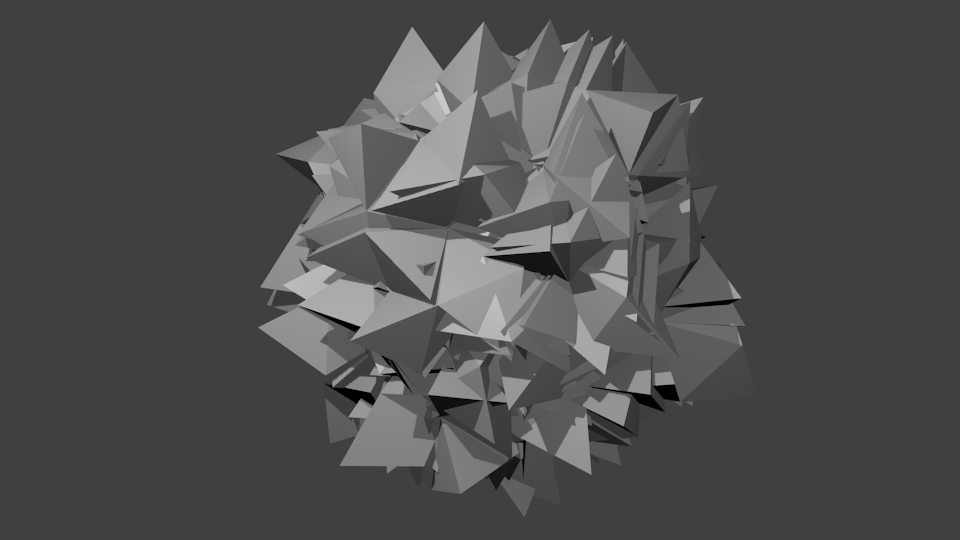
\includegraphics[width=.66\textwidth]{ball-grammar}
  \caption{An example of a ball shape commonly generated by a grammar}
  \label{fig:ball-gram}
\end{figure}

\par
Other known issues with the grammar is the abnormal behavior with Grow operations, in the negative direction.  As seen in Figure~\ref{fig:skewed-pyr}, on occasion when a Grow operation is performed on a face below the origin, it produces a skewed extension point, resulting in an irregular tetrahedron.  This behavior is obviously unwanted as the grammar works on the assumption that it operates on equilateral triangle faces, whereas those faces produced by the irregular Grow operations are not equilateral, which potentially causes issues with subsequent calculations.  More investigation is required in order to fix this, but the likely cause of this issue has to do with how faces are shifted towards the origin temporarily when a Grow operation is performed, in order to perform the calculations of the point extension.

\begin{figure}[h]
  \centering
  
\includegraphics[width=.66\textwidth]{skewed-faces}
  \caption{An irregular extension seemingly caused by an error in the calculations when Grow is called on a face oriented negative relative to the origin}
  \label{fig:skewed-pyr}
\end{figure}


\subsection{Implenting Evolutionary System}
Once the grammar system is fully functional, the basis for the evolutionary system will have to be implemented.  While we already have some basic grammar-randomization functionality, the implementation of the evolutionary operations will require further readings on the best practices when designing a Generative Encoding.  The most basic operations are trivial, such as mutating a genotype, which in essence is looking at a given grammar and deciding whether or not to change the Right Hand Side of any of its production rules.  Things will become more design intensive when more complicated evolutionary operations are implemented (e.g. Genetic Recombination of two highly-fit solutions), and the addition of the Generative Encoding aspect to the system (giving it the understanding of a particular sequence as a ``gene'').  Finally the design of the fitness functions (discussed below) will be a significant concern in the next steps of the project.

\subsection{Designing Measures of Fitness}
While we already have some basic ideas of measures of fitness based on some of the biological theories behind the evolution of skate intestines (e.g. the relationship between the volume of the shape and the surface area, the potential for water and protein absorbtion, etc.) designing the mathematic measures of fitness and extracting the relevant data from our models will require investigation moving forward.  Improving upon these basic measures of fitness to further biologically significant measures will require meeting with Professor Theodosiou in the Biology Department, who is heading the research into the study of skate gut morphologies and development.

%------------------------------------------------------------

\section{Evaluating Previous Proposal}
\par
Largely the work discussed in the proposal presented in the Spring has remained unchanged.  However some of the specifics, such as the actual system used, as well as the strength of the understanding of the goals of the project have changed.  The change in the grammar system came after the advisor to this project suggested looking at the tetrahedral grammar he had worked on for a previous project, as this provided a relatively simple to implement, robust, and interesting system.  The timeline has been shifted back fairly significantly as it was much harder to identify, and implement the systems needed, and moving forward there are potentially even more setbacks given the complexity of the math needed to create fitness functions and evaluate the results.  However, it seems as though it will still be possible to generate significant results by the end of Winter.

%------------------------------------------------------------

\bibliographystyle{plain}
\bibliography{centralbib}

\end{document}
